\documentclass[11pt]{article}
% Shared preamble for model_card.tex and assumptions_register.tex
\usepackage[T1]{fontenc}
\usepackage[utf8]{inputenc}
\usepackage{lmodern}
\usepackage[margin=2cm]{geometry}
\usepackage{amsmath,amssymb}
\usepackage{graphicx}
\usepackage{booktabs,longtable,tabularx,array,multirow}
\usepackage[table]{xcolor}
\usepackage{enumitem}
\usepackage{caption}
\usepackage[hidelinks]{hyperref}
\usepackage{xurl}
\usepackage{pdflscape}

\graphicspath{{figures/}}
\setlist{itemsep=2pt,topsep=3pt}
\captionsetup{font=small,labelfont=bf}
\renewcommand{\arraystretch}{1.15}

% ---- editing helpers -------------------------------------------------------
% \TODO{...} marks text the students still have to write or confirm (renders red in the PDF).
\newcommand{\TODO}[1]{\textcolor{red!75!black}{\textbf{[TODO:} #1\textbf{]}}}
% Single source for facts that appear in both documents; edit here, not in the text.
\newcommand{\Nall}{138{,}554}
\newcommand{\Nhh}{85{,}182}
\newcommand{\prev}{0.631}
\newcommand{\capacity}{30\%}
\newcommand{\epsTol}{0.10}
\newcommand{\minSupport}{30}
\newcommand{\nbDate}{25 October 2026}
% Team facts used by every document in writeup/, report/ and slides/. Edit here once.
\newcommand{\StudentA}{Sumedh Navuda}
\newcommand{\StudentB}{Aldino}
\newcommand{\Authors}{\StudentA{} and \StudentB{}}
\newcommand{\Contact}{sumedhnavuda@outlook.com}
\newcommand{\RollA}{[roll no.]}   % <- replace with Sumedh's roll number
\newcommand{\RollB}{[roll no.]}   % <- replace with Aldino's roll number
\newcommand{\RepoURL}{https://github.com/sumedhnvda/ict5143-p8-fairness-audits}
\newcommand{\TeamID}{[team ID]}   % <- replace with the team ID given by the instructor
\newcommand{\SubmitTag}{submission-v1}
   % names, roll numbers, contact, repository (shared with report/ and slides/)
\newcommand{\nb}{\texttt{Problem8\_\allowbreak Intersectional\_\allowbreak Fairness.ipynb}}
\newcommand{\sect}[1]{notebook~\S#1}
\newcommand{\status}[1]{\textsf{\small #1}}

\geometry{margin=2.3cm}
\linespread{1.0}
\usepackage{subcaption}

\title{When Does Pooling Make Intersectional Fairness Audits Falsely Reassuring?\\[3pt]
\large Bayesian audits of sparse race $\times$ sex $\times$ disability groups in ACSPublicCoverage}
\author{\Authors\\ \small \texttt{\EmailA}, \texttt{\EmailB} \quad \url{\RepoURL}\\ \small ICT 5143 Algorithms, Fairness and Graphical Models Laboratory --- Capstone, Problem 8}
\date{\nbDate}

\begin{document}
\maketitle

\begin{abstract}
Aggregate fairness audits can hide disparities at intersections of protected attributes. Intersections are often too
small for raw estimates, and hierarchical Bayesian pooling is the established remedy. We ask when such pooling makes an
audit \emph{falsely reassuring}, i.e.\ when it concludes that an equality-of-opportunity tolerance
$\Delta\text{EOpp}\le\epsilon$ holds when it does not. We use ACSPublicCoverage (California 2018; \Nall{} people), a
compact Bayesian-network predictor with exact inference, and a hypothetical outreach decision at 30\% capacity. We
compare raw, independent, exchangeable (empirical-Bayes and full-Bayes beta-binomial), attribute-structured (hierarchical
logistic) and $\epsilon$-contamination audits in synthetic, semi-synthetic and real experiments. Exchangeable pooling
declares a 0.20 deficit in a 24-positive intersection ``fair'' in 98--100\% of semi-synthetic worlds, and an
upper-posterior-quantile rule does not fix this. Attribute-structured pooling masks the same deficit when it is an
interaction. On real data, every one of 116 validation-time tolerance claims made by pooled criteria fails on an
independent household-disjoint test split (test $\Delta$EOpp 0.23--0.77). A contamination procedure calibrated on an invented design
lowers false claims, but its acceptance of truly fair worlds falls from 0.83 to 0.32 on the real design. We trace this to
groups with fewer than 10 positives and propose two fixes: \emph{design-matched calibration} on the deployment
population's own validation group sizes, and \emph{held-out certification}. In a preregistered out-of-sample test on
Texas 2018, the design-matched audit scores $J=\text{ACC}-\text{FTS}=0.664$, against at most 0.385 for every established
audit, at a false-certification rate of 0.168 (vs 0.615--0.661 for hierarchical pooling). Held-out certification removes
all validation-time false certificates (10 of 10 same-data claims were false; held-out certification made none). Our falsifiable claim (H1), that pooled validation-time tolerance claims fail on test more than half the time, is supported out of sample on Texas 2018 (27 of 27 claims failed).
\end{abstract}

\section{Introduction}
Fairness audits usually report one gap per protected attribute. Disadvantage, however, often concentrates at
intersections~\cite{kearns2018,wang2022}. Intersections of race, sex and disability are numerous and small, so raw
estimates of group true-positive rates (TPRs) are noisy and the max$-$min gap is biased upward~\cite{lum2022}.
Hierarchical Bayesian models stabilise such estimates by partial pooling~\cite{foulds2020bayes,ji2020,herlihy2024}.
Pooling, however, pulls a small group toward the majority. If that group is the one that is actually disadvantaged, the
audit may certify fairness that does not exist.

\paragraph{Research questions.} \textbf{RQ1:} When does hierarchical pooling improve intersectional fairness
assessment, and when does it mask a harmful small-group disparity? \textbf{RQ2:} How do pooling strength and group size
affect interval coverage? \textbf{RQ3:} Can posterior uncertainty (an upper posterior quantile) improve validation-time
threshold selection? \textbf{RQ4:} Are conclusions stable across splits and populations?

\paragraph{Contributions.} The literature already establishes hierarchical intersectional estimation, small-group
unreliability, marginal-vs-intersectional gaps and contamination priors (Section~\ref{sec:related}). We therefore claim
an \emph{evaluation}, not a new estimator:
(i) a controlled comparison of false tolerance-satisfaction rates (FTS) for six audit families, under minority thinning
and three deficit structures, on both an invented and the real intersection design;
(ii) evidence that pooled audit criteria used for validation-time rule selection make tolerance claims that fail on
independent data;
(iii) a diagnosis of why a simulation-calibrated robust-prior procedure fails to transfer between designs, and a fix,
\emph{design-matched calibration plus held-out certification}, tested out of sample with preregistered hypotheses
(H2a--c); and
(iv) an out-of-sample test, on a second state, of the falsifiable claim

\begin{quote}\textbf{H1.} \emph{When the group-threshold rule's $\lambda$ is selected on validation data and a pooled
Bayesian audit criterion reports intersectional $\Delta\text{EOpp}\le0.10$, the frozen rule's empirical test
$\Delta\text{EOpp}$ exceeds 0.10 in more than half of those cases.}\end{quote}

\section{Related work}\label{sec:related}
\emph{Intersectional definitions.} Subgroup fairness over rich classes~\cite{kearns2018}, multicalibration~\cite{hebert2018}
and differential fairness~\cite{foulds2020icde} formalise intersectional fairness. Marginal fairness does not in general
imply intersectional fairness~\cite{molina2022}; a survey is given in~\cite{gohar2023}.
\emph{Small-group estimation.} Foulds et al.~\cite{foulds2020bayes} introduce Bayesian models, including a hierarchical
Bayesian logistic regression, for sparse intersections. Ji et al.~\cite{ji2020} estimate fairness metrics with a
hierarchical Bayesian calibration model. Herlihy et al.~\cite{herlihy2024} use structured regression with confidence
intervals for very small subgroups. Lum et al.~\cite{lum2022} show that naive disparity estimates are biased.
Himmelreich et al.~\cite{himmelreich2025} frame intersectionality as a problem of statistical uncertainty. Morina et
al.~\cite{morina2019} extend audit metrics to intersections.
\emph{Inference and generalisation.} Cherian and Cand\`es~\cite{cherian2024} give simultaneous bootstrap bounds for
subgroup audits. Cotter et al.~\cite{cotter2019} show that fairness constraints may not generalise and enforce them on
validation data. Hardt et al.~\cite{hardt2016} define equality of opportunity and threshold post-processing.
\emph{Robust shrinkage.} $\epsilon$-contaminated priors~\cite{berger1986} and heavy-tailed hierarchical priors for outlying
small areas~\cite{datta1995} are classical.
\emph{Data and labels.} We use Folktables~\cite{ding2021,folktables}; label noise can overturn fairness
conclusions~\cite{fogliato2020}. The full review, with a comparison table of 19 papers, is in the companion document
\texttt{literature\_review.pdf}.

\section{Data, decision and metrics}
\textbf{Data.} ACS PUMS 2018 1-Year, California, through Folktables' \texttt{ACSPublicCoverage} task (AGEP $<65$, PINCP
$\le30{,}000$): \Nall{} people in \Nhh{} households, 19 features identical to Folktables' output. The label is
$Y=1-\mathbb 1[\text{PUBCOV}=1]$ (prevalence \prev): $Y=1$ means \emph{no public coverage}, which is neither uninsurance
nor eligibility. Protected attributes are RAC1P (nine codes, not collapsed), SEX and DIS, giving 36 intersections. Splits
are household-disjoint 60/20/20 on SERIALNO with five seeds. Texas 2018 (98,928 people) is a replication population.

\textbf{Decision.} $D=1$ selects a person for \emph{hypothetical} information outreach, at a fixed capacity of 30\%.
The rule family is $t_g(\lambda)=(1-\lambda)t_{\text{global}}+\lambda t_g^{\text{EOpp}}+c$, with $c$ chosen so that exactly
30\% of validation records are selected. $\lambda=0$ is group-unaware; $\lambda=1$ is ordinary opportunity-constrained
threshold adjustment~\cite{hardt2016}.

\textbf{Metrics (preregistered).} The primary fairness metric is intersectional
$\Delta\text{EOpp}=\max_g t_g-\min_g t_g$ over groups with $\ge30$ positives, with tolerance $\epsilon=0.10$ (robustness
0.05 and 0.15). The primary predictive metric is recall at capacity, with an acceptable utility loss of 0.02. $\Delta$DP,
$\Delta$EOdds, $R_{\text{sel}}$, worst-group recall, AUROC, AP, log loss, Brier score and group calibration are
diagnostics. In simulation we report FTS $=P(\text{declared fair}\mid\text{truly unfair})$, ACC
$=P(\text{declared fair}\mid\text{truly fair})$, and the coverage and width of central 90\% intervals.

\section{Methods}
\subsection{Predictive Bayesian network and exact inference}
The predictor is a discrete augmented naive-Bayes network: $Y$ is a parent of all 18 features, plus edges such as
PINCP$\mid$ESR and \{DEAR, DEYE, DREM\}$\mid$DIS (Figure~\ref{fig:models}a). CPTs are Dirichlet-smoothed ($\alpha=1$) and
$P(Y\mid x)$ is computed by variable elimination. Across 200 random evidence masks, our VE under two elimination orders,
pgmpy VE, pgmpy clique-tree belief propagation and enumeration agree to $3.3\times10^{-16}$. The joint conditional
independence $\text{SEX}\perp\{\text{AGEP},\text{DIS}\}\mid Y$ implied by d-separation holds in the fitted model. The
graph is associational. Logistic regression and gradient-boosted trees are predictive baselines.

\begin{figure}[t]\centering
\begin{subfigure}{0.5\textwidth}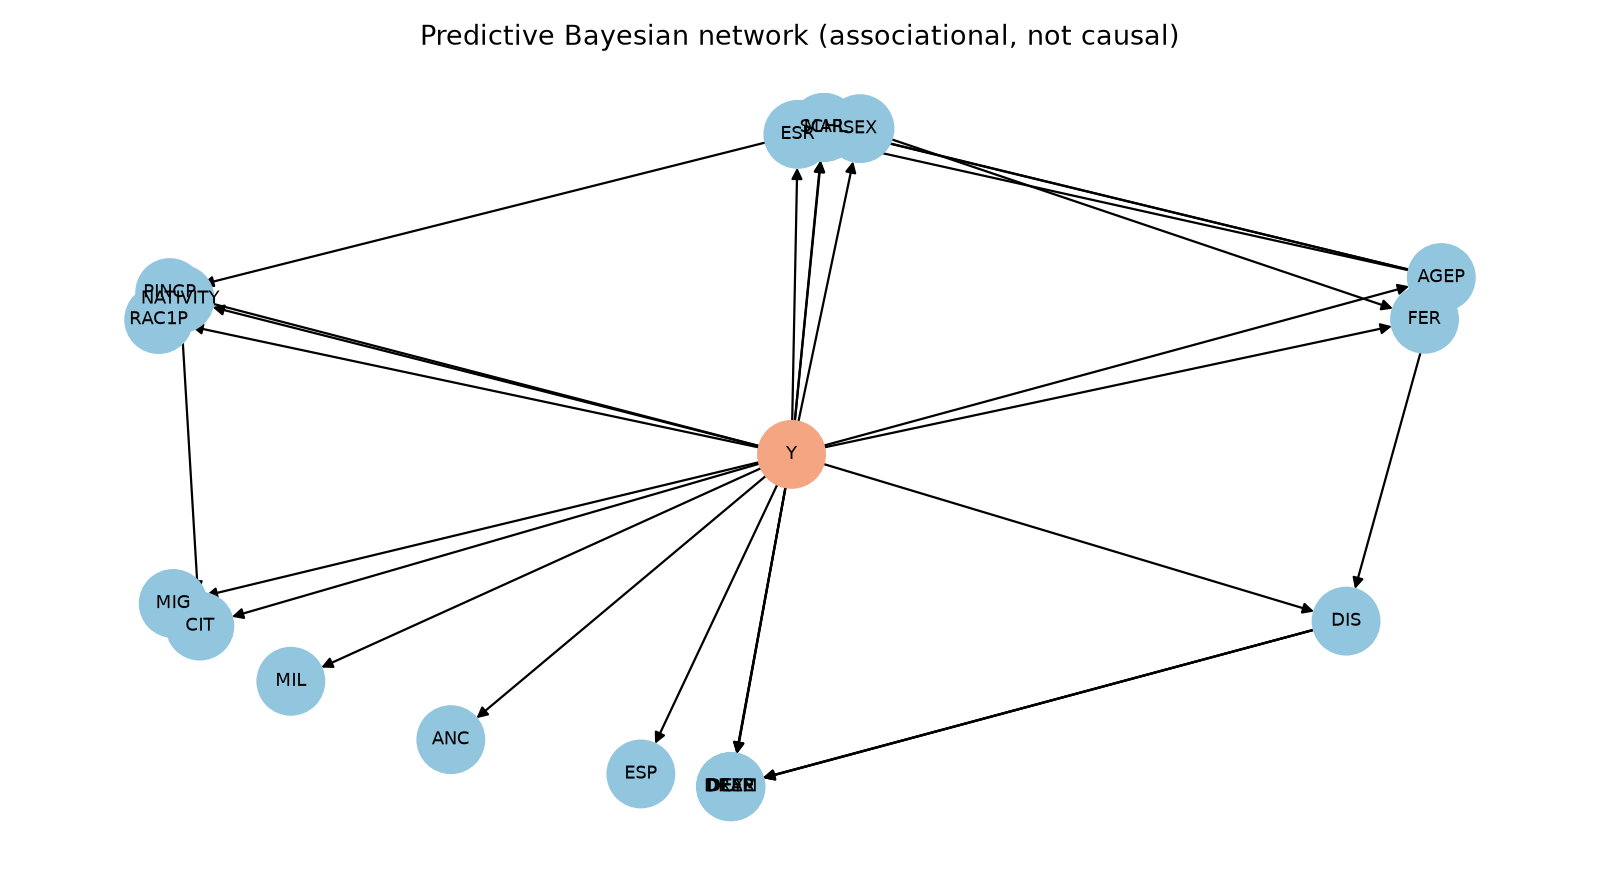
\includegraphics[width=\linewidth]{bn_structure.png}\caption{Predictive BN}\end{subfigure}\hfill
\begin{subfigure}{0.47\textwidth}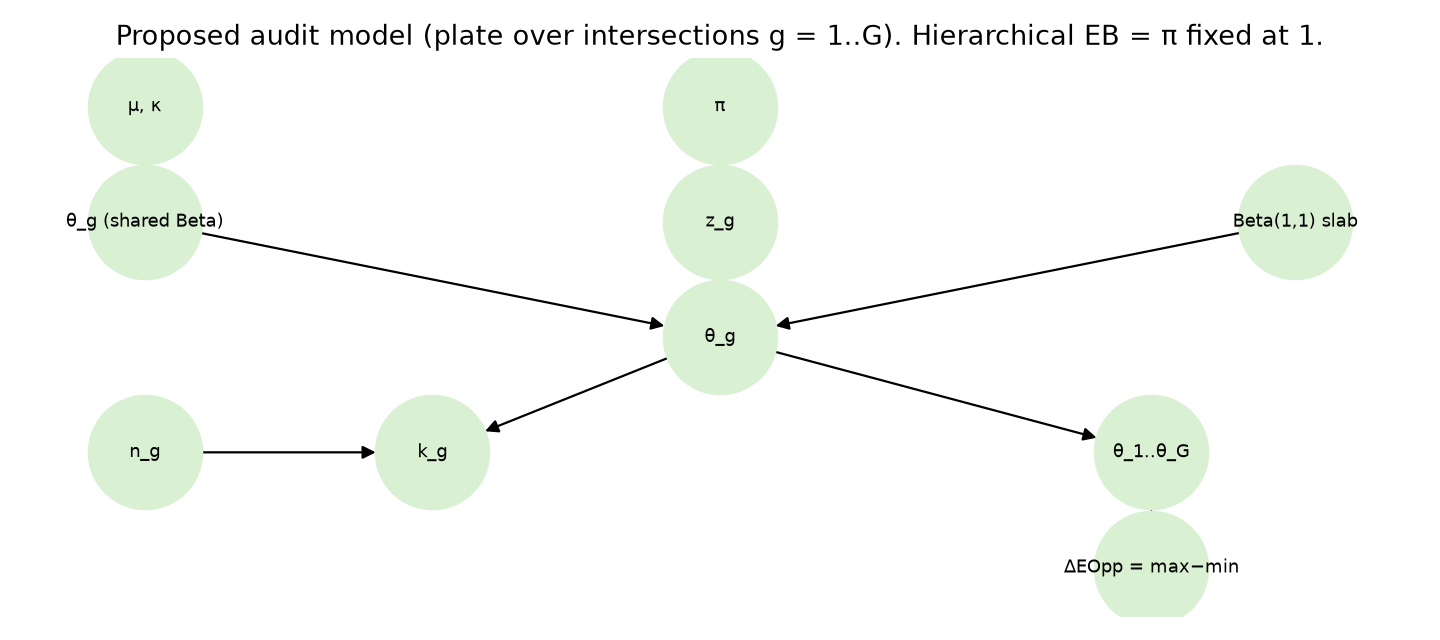
\includegraphics[width=\linewidth]{audit_model_structure.png}\caption{Contamination audit model}\end{subfigure}
\caption{Graphical models. (a) Associational predictor. (b) Audit model with a plate over intersections; hierarchical
EB is the special case $\pi=1$.}\label{fig:models}
\end{figure}

\subsection{Audit models}
For a frozen rule, let $n_g$ be the positives in intersection $g$ and $k_g$ the selected positives, with
$k_g\sim\text{Bin}(n_g,\theta_g)$ and $\theta_g$ the TPR. We compare:
\emph{raw} $k_g/n_g$;
\emph{independent} $\theta_g\sim\text{Beta}(1,1)$ (no pooling);
\emph{complete} pooling (one shared $\theta$);
\emph{hier}, $\theta_g\sim\text{Beta}(a,b)$ with $(a,b)$ fitted by beta-binomial marginal likelihood;
\emph{fullbayes}, $\text{Beta}(\mu\kappa,(1-\mu)\kappa)$ with $\mu\sim U(0,1)$, $p(\kappa)\propto(1+\kappa)^{-2}$, on a grid;
\emph{struct}, the attribute-structured hierarchical logistic audit
$\operatorname{logit}\theta_g=\beta_0+\beta_{\text{race}}+\beta_{\text{sex}}+\beta_{\text{dis}}+u_g$,
$u_g\sim N(0,\tau^2)$, with $(\beta,\tau)$ fitted by marginal likelihood using 201-node adaptive quadrature (a restricted
version in the spirit of~\cite{foulds2020bayes}, not an exact reproduction); and
\emph{contamination}, $\theta_g\sim\pi\,\text{Beta}(a,b)+(1-\pi)\,\text{Beta}(1,1)$ with $\pi\le\pi_{\max}$~\cite{berger1986}.
Under the contamination prior the posterior is a two-component Beta mixture, so a group whose counts are implausible
under the shared Beta keeps its own estimate. A \emph{plug-in} rule declares fairness if the max$-$min of the posterior
means is $\le\epsilon$. An \emph{upper-$q$} rule declares fairness if the $q$-quantile of the posterior of
$\max_g\theta_g-\min_g\theta_g$ is $\le\epsilon$, equivalently $P(\Delta>\epsilon\mid\text{data})\le1-q$.

\subsection{Calibrating the tolerance procedure}
Before any real-data selection, we chose the audit procedure on synthetic data with a preregistered rule: maximise
Youden's $J=\text{ACC}-\text{FTS}$ over (estimator, rule) pairs. The synthetic design has 16 intersections with
4000 down to 8 positives, homogeneous TPRs $0.65\pm0.015$, and in the unfair worlds one 20-positive group 0.20 lower,
with $R=300$ replicates. The chosen procedure is then frozen.

\subsection{Experiments}
\textbf{E1} compares single-attribute, two-attribute and intersectional audits.
\textbf{E2} thins three disabled minority intersections in training and validation to 50, 25 and 10\% while keeping the
test split intact.
\textbf{E3} compares raw, independent and pooled estimates on real counts.
\textbf{E4} simulates homogeneous and exceptional worlds on the synthetic design and, \emph{semi-synthetically}, on the real
seed-0 validation design (32 intersections, 1 to 5,499 positives). The deficit sits at Black, female, disabled
(\texttt{2|2|1}, 24 positives), thinned to 100, 50 and 25\%, and takes three forms: an isolated \emph{cell}; a pure
\emph{interaction}, in which the other 31 groups are shifted so that every race, sex and disability margin is exactly
equal; and a \emph{disability main effect}.
\textbf{E5} selects $\lambda$ on validation with each criterion (raw, independent, complete, hier, fullbayes, struct and
contamination; plug-in and upper rules) and audits the frozen rule on test, with capacity matched.
Ablations remove pooling, use complete pooling, and replace the upper quantile by the posterior mean. Robustness tests vary
priors and $\pi_{\max}$, base TPR, $\epsilon$, effect size and thinning, and add survey weights and Texas.
\textbf{Statistics.} Evaluation uncertainty comes from 1,000 household-cluster bootstrap replicates of the seed-0 test
split. Training uncertainty comes from 5 refits. The confirmatory family (Holm) is the calibrated procedure vs hier
plug-in and vs raw plug-in, on test $\Delta$EOpp. Everything else is exploratory.

\section{Results}
\subsection{Intersectional audits reveal what single attributes hide (E1)}
Predictive accuracy is moderate: BN AUROC $0.729\pm0.004$, LR $0.716\pm0.004$, GBT $0.768\pm0.003$
(Table~\ref{tab:pred}). For the unconstrained BN rule, $\Delta$EOpp is 0.162 by sex, 0.384 by disability, 0.468 for
sex$\times$disability and \textbf{0.746 intersectionally} (21 of 35 groups adequate; Table~\ref{tab:exp1}). Every disabled
intersection has a TPR of at most 0.08. Disabled low-income adults mostly do have public coverage, so the minority of them
without it is ranked low. Survey weighting confirms this (weighted TPR 0.011 and 0.031 for disabled men and women, against
0.280 and 0.448 without a disability). Texas replicates the pattern (0.094 by sex; 0.888 intersectionally).

\begin{table}[t]\centering\small
\caption{Test metrics of the unconstrained top-30\% rule (mean $\pm$ sd over 5 household splits).}\label{tab:pred}
% generated by make_tables.py from ../results; do not edit by hand
\begin{tabular}{lccc}
\toprule
Metric & BN & LR & GBT \\
\midrule
AUROC & 0.729 $\pm$ 0.004 & 0.716 $\pm$ 0.004 & 0.768 $\pm$ 0.003 \\
AP & 0.803 $\pm$ 0.002 & 0.787 $\pm$ 0.002 & 0.836 $\pm$ 0.002 \\
Recall@30\% & 0.388 $\pm$ 0.005 & 0.384 $\pm$ 0.006 & 0.409 $\pm$ 0.006 \\
Prec.@30\% & 0.824 $\pm$ 0.004 & 0.809 $\pm$ 0.004 & 0.860 $\pm$ 0.002 \\
Log loss & 0.577 $\pm$ 0.004 & 0.584 $\pm$ 0.002 & 0.541 $\pm$ 0.003 \\
Brier & 0.196 $\pm$ 0.002 & 0.199 $\pm$ 0.001 & 0.182 $\pm$ 0.001 \\
max group ECE & 0.110 $\pm$ 0.010 & 0.069 $\pm$ 0.011 & 0.063 $\pm$ 0.013 \\
$\Delta$EOpp & 0.719 $\pm$ 0.018 & 0.625 $\pm$ 0.049 & 0.585 $\pm$ 0.019 \\
$\Delta$DP & 0.655 $\pm$ 0.016 & 0.548 $\pm$ 0.021 & 0.508 $\pm$ 0.013 \\
worst recall & 0.000 $\pm$ 0.000 & 0.000 $\pm$ 0.000 & 0.008 $\pm$ 0.011 \\
\bottomrule
\end{tabular}

\end{table}
\begin{table}[t]\centering\small
\caption{Single-attribute vs intersectional audit (seed-0 test split, unconstrained rule).}\label{tab:exp1}
\resizebox{\textwidth}{!}{% generated by make_tables.py from ../results; do not edit by hand
\begin{tabular}{lc*{9}{c}}
\toprule
& & \multicolumn{3}{c}{BN} & \multicolumn{3}{c}{LR} & \multicolumn{3}{c}{GBT} \\
\cmidrule(lr){3-5}\cmidrule(lr){6-8}\cmidrule(lr){9-11}
Grouping & adequate/all & $\Delta$EOpp & $\Delta$DP & worst rec. & $\Delta$EOpp & $\Delta$DP & worst rec. & $\Delta$EOpp & $\Delta$DP & worst rec. \\
\midrule
SEX & 2/2 & 0.162 & 0.128 & 0.291 & 0.080 & 0.060 & 0.338 & 0.095 & 0.077 & 0.346 \\
DIS & 2/2 & 0.384 & 0.324 & 0.021 & 0.396 & 0.334 & 0.010 & 0.354 & 0.307 & 0.067 \\
RACE & 8/9 & 0.597 & 0.548 & 0.079 & 0.561 & 0.456 & 0.106 & 0.360 & 0.313 & 0.169 \\
SEX$\times$DIS & 4/4 & 0.468 & 0.386 & 0.009 & 0.436 & 0.361 & 0.004 & 0.427 & 0.352 & 0.034 \\
RACE$\times$SEX & 14/18 & 0.678 & 0.614 & 0.059 & 0.611 & 0.517 & 0.099 & 0.429 & 0.410 & 0.155 \\
RACE$\times$DIS & 13/18 & 0.697 & 0.634 & 0.000 & 0.686 & 0.554 & 0.000 & 0.544 & 0.464 & 0.000 \\
RACE$\times$SEX$\times$DIS & 21/35 & 0.746 & 0.683 & 0.000 & 0.711 & 0.580 & 0.000 & 0.600 & 0.519 & 0.000 \\
\bottomrule
\end{tabular}
}
\end{table}

\subsection{Pooling on real counts (E3)}
On real counts the exchangeable estimators move only groups with 1--7 positives (pull 0.05--0.14), and no group with
$\ge30$ positives moves by more than 0.032 (Figure~\ref{fig:pull}). The TPRs are bimodal by disability, so the shared Beta
is diffuse. The struct model fits $\hat\tau=0.01$ (its lower bound), so it becomes a main-effects model with an implausibly
narrow gap interval, (0.750, 0.757). Every audit gives $P(\Delta\text{EOpp}>0.10\mid\text{data})=1.0$, so here pooling neither
hides the disparity nor needs correcting.

\begin{figure}[t]\centering
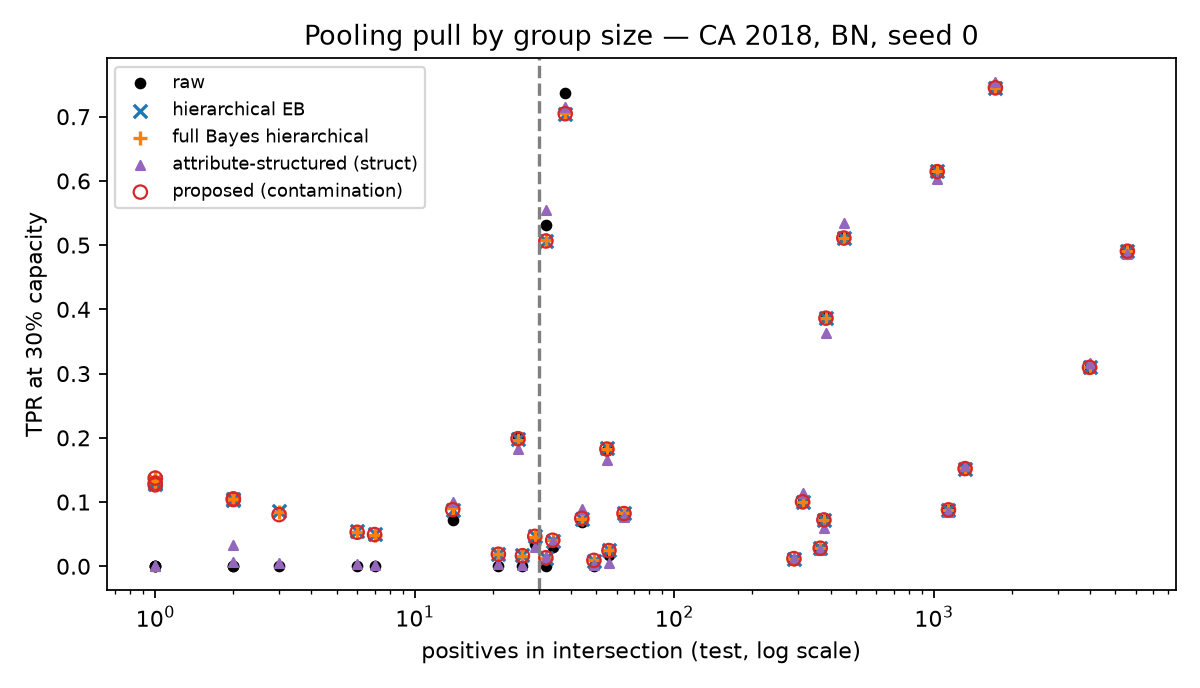
\includegraphics[width=0.66\textwidth]{real_pooling_pull.png}
\caption{Raw and pooled TPR estimates by intersection size (BN, seed 0, test).}\label{fig:pull}
\end{figure}

\subsection{Pooling masks a small exception; quantile rules do not fix it (E4, SYNTHETIC)}
Table~\ref{tab:sim} and Figure~\ref{fig:frontiers}a summarise the synthetic study. Empirical-Bayes pooling declares the
unfair worlds fair in 100\% (plug-in) and 98\% (upper 0.9) of replicates, because shrinkage moves the exceptional group's
posterior location, not just its interval width. Full Bayes with the upper 0.9 rule lowers FTS to 0.31, but accepts only
43\% of fair worlds. Raw and independent audits never certify (ACC $\le0.007$). No configuration achieves FTS $<0.10$
with ACC $>0.5$. The preregistered calibration selected the contamination prior with $\pi_{\max}=0.8$ and the
\emph{plug-in} rule (FTS 0.503, ACC 0.830, $J=0.327$). The best upper-quantile rule ($J=0.323$) is within Monte Carlo
error, so for RQ3 posterior quantiles did not improve the calibrated choice. Coverage of the 90\% gap interval is 0.000 for
hier and 0.038 for full Bayes, against 0.962 for the calibrated contamination prior. For RQ2, the struct audit under its
own generative model covers only 0.665 at nominal 0.90 (0.53 for groups with $<30$ positives). With the true
hyperparameters the same sampler gives 0.905, so the shortfall comes from empirical-Bayes plug-in estimation.

\begin{table}[t]\centering\small
\caption{SYNTHETIC: FTS by thinning of the exceptional group, ACC, and 90\% gap-interval coverage and width ($R=300$).}\label{tab:sim}
% generated by make_tables.py from ../results; do not edit by hand
\begin{tabular}{lcccccc}
\toprule
& \multicolumn{3}{c}{FTS (exceptional group kept)} & ACC & \multicolumn{2}{c}{90\% gap interval} \\
\cmidrule(lr){2-4}\cmidrule(lr){6-7}
Estimator $\cdot$ rule & 100\% & 50\% & 25\% & homog. & coverage & width \\
\midrule
raw $\cdot$ plugin & 0.003 & 0.000 & 0.000 & 0.007 & -- & -- \\
independent $\cdot$ upper 0.9 & 0.000 & 0.000 & 0.000 & 0.000 & 0.264 & 0.382 \\
complete $\cdot$ plugin & 1.000 & 1.000 & 1.000 & 1.000 & 0.000 & 0.000 \\
hier $\cdot$ plugin & 1.000 & 1.000 & 1.000 & 1.000 & 0.000 & 0.018 \\
hier $\cdot$ upper 0.9 & 0.980 & 0.987 & 0.987 & 0.993 & 0.000 & 0.018 \\
fullbayes $\cdot$ plugin & 0.983 & 1.000 & 0.993 & 1.000 & 0.038 & 0.114 \\
fullbayes $\cdot$ upper 0.9 & 0.310 & 0.337 & 0.397 & 0.427 & 0.038 & 0.114 \\
\textbf{proposed $\pi\le$0.8 $\cdot$ plugin (calibrated)} & 0.503 & 0.593 & 0.563 & 0.830 & 0.962 & 0.399 \\
proposed $\pi\le$0.8 $\cdot$ upper 0.5 & 0.450 & 0.567 & 0.577 & 0.773 & 0.962 & 0.399 \\
proposed $\pi\le$0.8 $\cdot$ upper 0.9 & 0.000 & 0.000 & 0.000 & 0.000 & 0.962 & 0.399 \\
proposed $\pi\le$0.95 $\cdot$ upper 0.9 & 0.297 & 0.300 & 0.317 & 0.527 & 0.589 & 0.273 \\
proposed $\pi\le$0.99 $\cdot$ upper 0.9 & 0.780 & 0.830 & 0.883 & 0.930 & 0.200 & 0.114 \\
\bottomrule
\end{tabular}

\end{table}

\begin{figure}[t]\centering
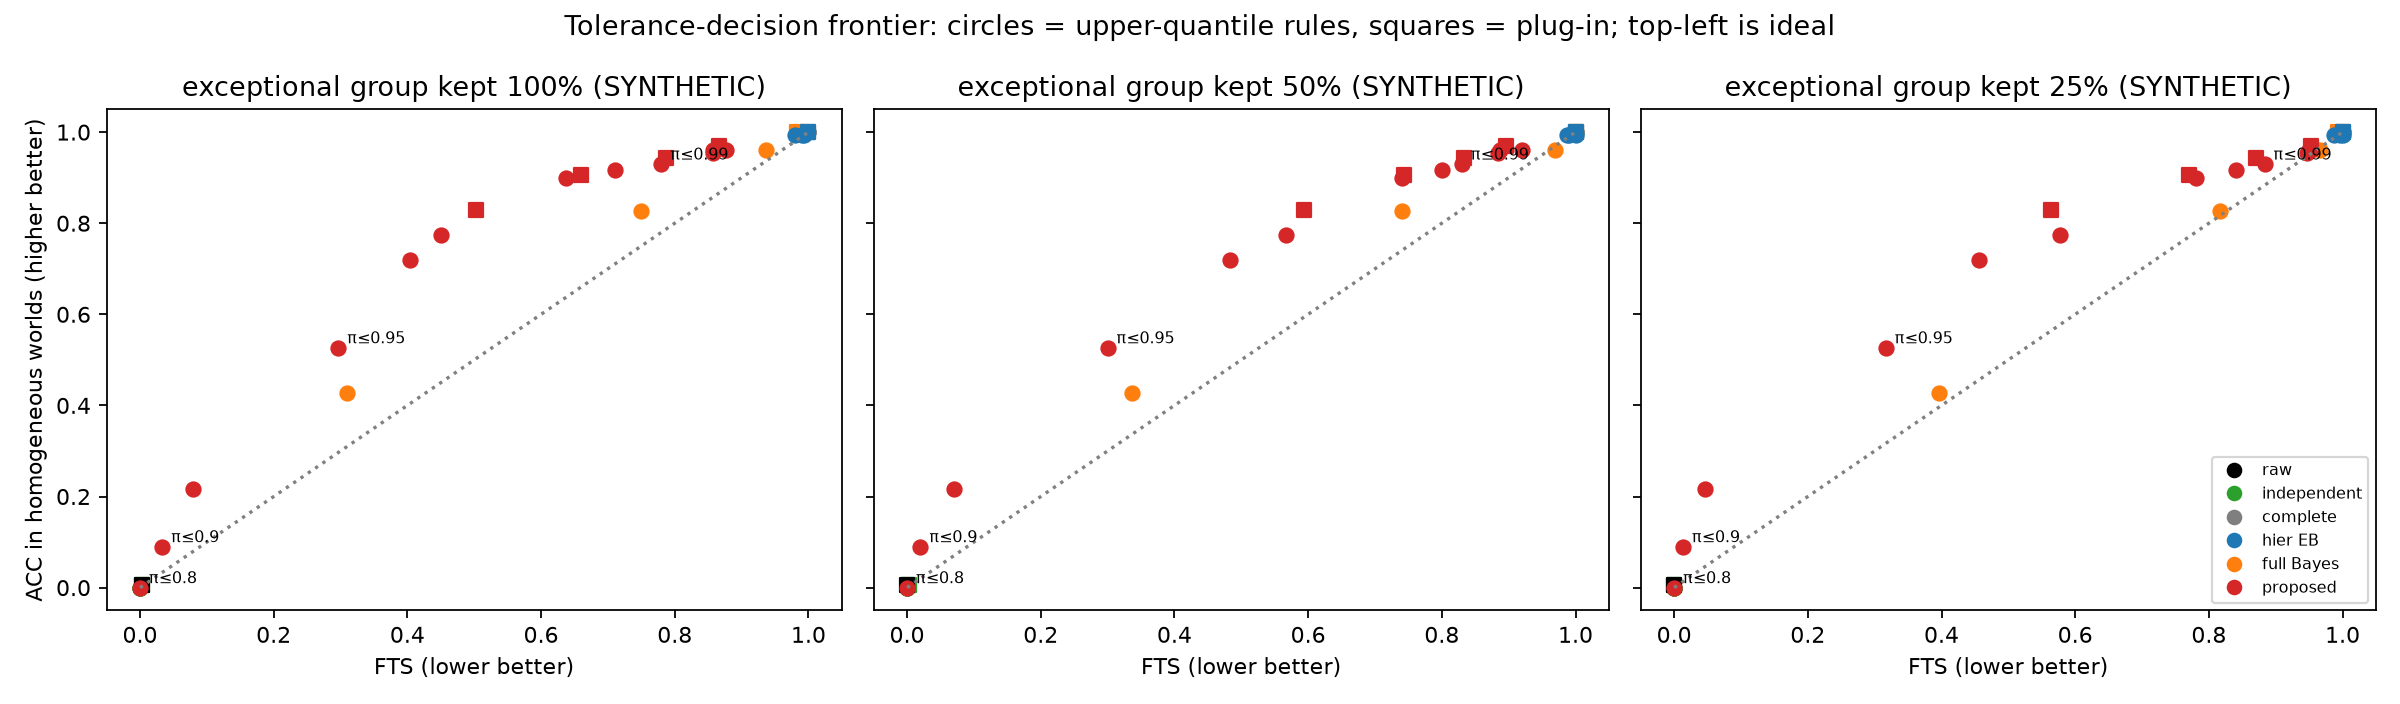
\includegraphics[width=0.86\textwidth]{sim_frontier.png}\\[2pt]
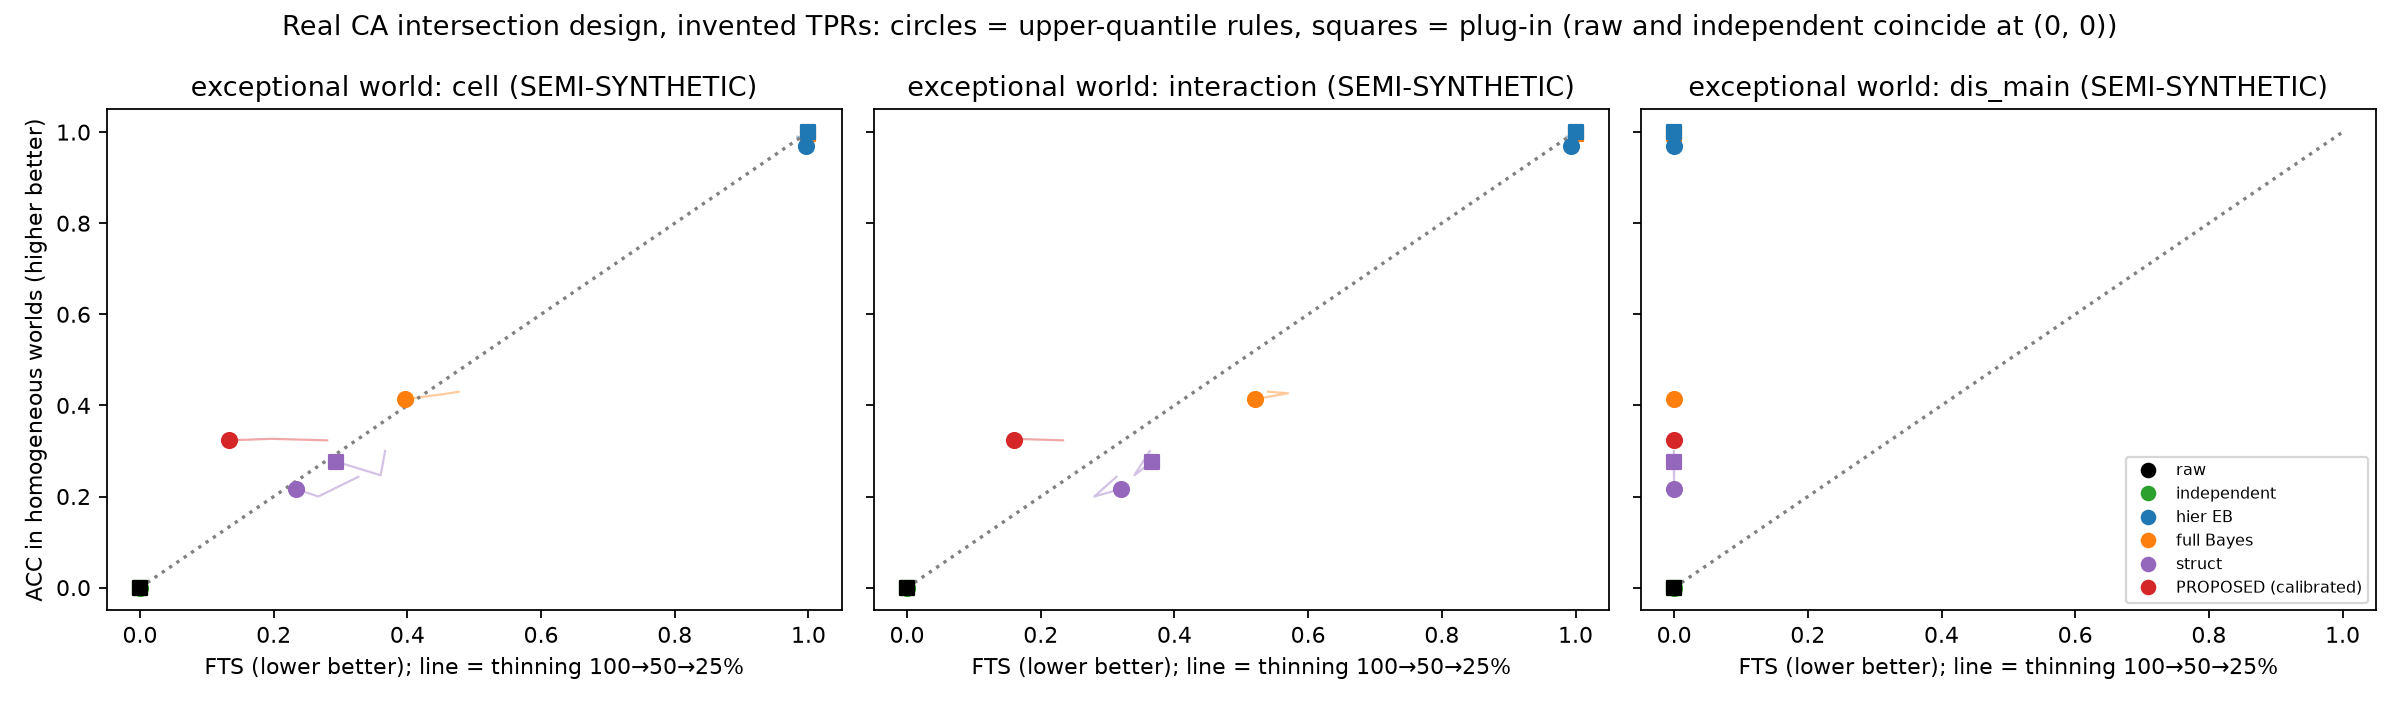
\includegraphics[width=0.86\textwidth]{semisynthetic_frontier.png}
\caption{Tolerance-decision frontiers (top-left is ideal). Top: SYNTHETIC design. Bottom: SEMI-SYNTHETIC worlds on the
real CA design, by deficit structure.}\label{fig:frontiers}
\end{figure}

\subsection{On the real design: structure of the deficit matters, and calibration does not transfer (E4, SEMI-SYNTHETIC)}
Table~\ref{tab:semi} gives the results on the real design. Hier declares the 24-positive cell deficit fair in 98--100\% of
worlds, and its posterior mean for \texttt{2|2|1} is 0.378 against a truth of 0.18. The attribute-structured audit also
masks the deficit when it is an isolated cell or a pure interaction: its mean is 0.368--0.377, its interval coverage for
\texttt{2|2|1} is 0.000 and its FTS is 0.23--0.37. When the deficit is a disability main effect shared by all 16 disabled
groups, every estimator detects it. The calibrated procedure keeps FTS at 0.13--0.28 (higher with thinning), but its ACC
is 0.32, against 0.83 in calibration. Many tiny groups give some group a chance to escape pooling in most fair worlds.

\begin{table}[t]\centering\small
\caption{SEMI-SYNTHETIC (real seed-0 validation design, invented TPRs; $R=300$).}\label{tab:semi}
\resizebox{\textwidth}{!}{% generated by make_tables.py from ../results; do not edit by hand
\begin{tabular}{lcccccccc}
\toprule
& ACC & \multicolumn{2}{c}{FTS cell} & \multicolumn{2}{c}{FTS interaction} & FTS dis. & \multicolumn{2}{c}{$\theta_{2|2|1}$ (cell, keep 1)} \\
\cmidrule(lr){3-4}\cmidrule(lr){5-6}\cmidrule(lr){8-9}
Procedure & keep 1 & keep 1 & keep .25 & keep 1 & keep .25 & keep 1 & 90\% cov. & post. mean \\
\midrule
\textbf{proposed (robust@0.8, plugin)} & 0.323 & 0.133 & 0.280 & 0.160 & 0.233 & 0.000 & 0.720 & 0.281 \\
fullbayes $\cdot$ plugin & 0.997 & 1.000 & 0.997 & 1.000 & 1.000 & 0.000 & 0.000 & 0.371 \\
fullbayes $\cdot$ upper0.9 & 0.413 & 0.397 & 0.477 & 0.520 & 0.540 & 0.000 & 0.000 & 0.371 \\
hier $\cdot$ plugin & 1.000 & 1.000 & 0.997 & 1.000 & 1.000 & 0.000 & 0.000 & 0.378 \\
hier $\cdot$ upper0.9 & 0.970 & 0.997 & 0.983 & 0.993 & 0.987 & 0.000 & 0.000 & 0.378 \\
independent $\cdot$ plugin & 0.000 & 0.000 & 0.000 & 0.000 & 0.000 & 0.000 & 0.900 & 0.201 \\
independent $\cdot$ upper0.9 & 0.000 & 0.000 & 0.000 & 0.000 & 0.000 & 0.000 & 0.900 & 0.201 \\
raw $\cdot$ plugin & 0.000 & 0.000 & 0.000 & 0.000 & 0.000 & 0.000 & -- & -- \\
struct $\cdot$ plugin & 0.277 & 0.293 & 0.367 & 0.367 & 0.363 & 0.000 & 0.000 & 0.368 \\
struct $\cdot$ upper0.9 & 0.217 & 0.233 & 0.327 & 0.320 & 0.313 & 0.000 & 0.000 & 0.368 \\
\bottomrule
\end{tabular}
}
\end{table}

\subsection{Validation-time tolerance claims fail on test (E2, E5)}
Table~\ref{tab:sel} gives the selection results. Pooled criteria (hier, full Bayes, complete, the calibrated contamination
rule, and struct in 2 of 5 splits) found a $\lambda$ satisfying $\epsilon=0.10$ on validation. Raw and independent criteria
never did. \textbf{All 116 pooled claims across splits and thinning levels failed on the test split}, with test
$\Delta$EOpp from 0.227 to 0.770. Part of this is pooling and part is that thresholds fitted on small validation
intersections do not transfer: the raw validation gap at $\lambda=1$ is 0.48. Thinning to 10\% raises the mean test gap
to 0.376--0.410. Utility is within budget: recall is 0.388 at $\lambda=0$ and 0.380 at $\lambda=1$ (the cost is at most
0.013 in any split). Figure~\ref{fig:tradeoff} shows the trade-off curves.

\begin{table}[t]\centering\small
\caption{Rule selection on validation, audited on test (intact data, 5 splits).}\label{tab:sel}
\resizebox{\textwidth}{!}{% generated by make_tables.py from ../results; do not edit by hand
\begin{tabular}{lcccccccc}
\toprule
Selection criterion & feasible on val. & mean $\lambda$ & test recall & test sel. rate & test $\Delta$EOpp (mean $\pm$ sd) & worst recall & test $P(\Delta>\epsilon)$ \\
\midrule
raw $\cdot$ plug-in & 0/5 & 0.80 & 0.385 & 0.299 & 0.348 $\pm$ 0.077 & 0.172 & 0.997 \\
independent $\cdot$ upper & 0/5 & 0.84 & 0.383 & 0.299 & 0.418 $\pm$ 0.094 & 0.191 & 0.996 \\
complete $\cdot$ plug-in & 5/5 & 0.26 & 0.390 & 0.298 & 0.641 $\pm$ 0.066 & 0.019 & 1.000 \\
hier EB $\cdot$ plug-in & 5/5 & 0.90 & 0.383 & 0.299 & 0.323 $\pm$ 0.077 & 0.210 & 0.965 \\
hier EB $\cdot$ upper & 5/5 & 1.00 & 0.380 & 0.299 & 0.367 $\pm$ 0.060 & 0.260 & 0.952 \\
full Bayes $\cdot$ upper & 5/5 & 1.00 & 0.380 & 0.299 & 0.367 $\pm$ 0.060 & 0.260 & 0.950 \\
struct $\cdot$ plug-in & 2/5 & 1.00 & 0.380 & 0.299 & 0.367 $\pm$ 0.060 & 0.260 & 0.955 \\
struct $\cdot$ upper & 2/5 & 1.00 & 0.380 & 0.299 & 0.367 $\pm$ 0.060 & 0.260 & 0.950 \\
\textbf{proposed $\cdot$ plug-in (calibrated)} & 5/5 & 0.96 & 0.381 & 0.299 & 0.332 $\pm$ 0.072 & 0.245 & 0.921 \\
proposed $\cdot$ upper & 0/5 & 1.00 & 0.380 & 0.299 & 0.367 $\pm$ 0.060 & 0.260 & 0.952 \\
\bottomrule
\end{tabular}
}
\end{table}

\begin{figure}[t]\centering
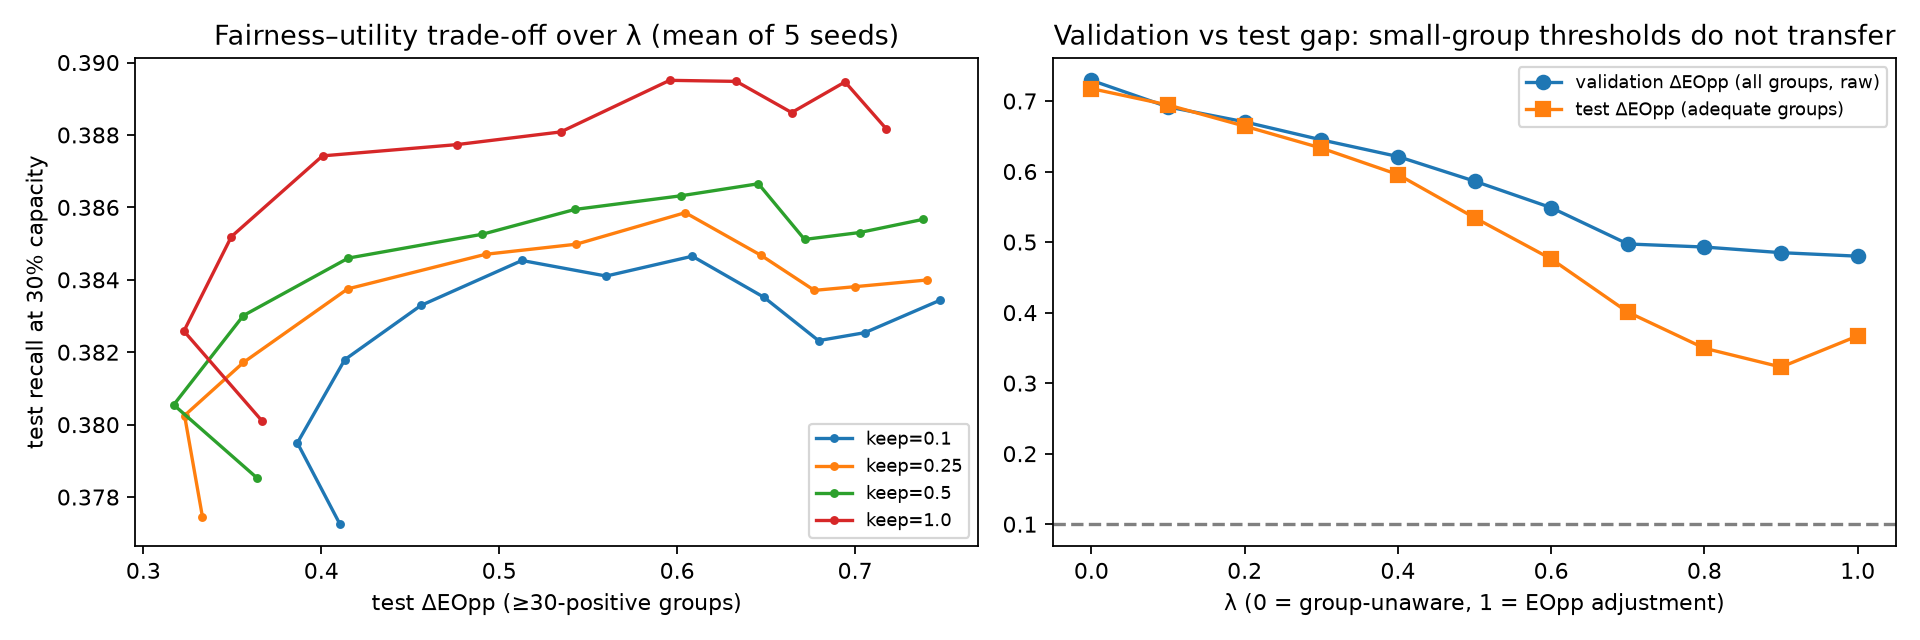
\includegraphics[width=0.85\textwidth]{tradeoff_curves.png}
\caption{Fairness--utility trade-off over $\lambda$ (left) and validation vs test gap (right), mean of 5 splits.}\label{fig:tradeoff}
\end{figure}

\subsection{Confirmatory tests, refits and out-of-sample test of H1 (RQ4)}
In the seed-0 bootstrap ($B=1000$), the calibrated procedure and hier plug-in chose the same $\lambda=0.9$ (difference
exactly 0; Holm $p=1$). Against raw plug-in the test $\Delta$EOpp difference is $-0.052$, 95\% CI $[-0.194,0.051]$, Holm
$p=0.736$, at a recall cost of $-0.006$ $[-0.0089,-0.0035]$. Across the 5 refits the paired differences change sign
($-0.016\pm0.039$ vs raw; $+0.009\pm0.035$ vs hier), so neither evaluation nor training uncertainty supports an
improvement. An earlier seed-0 result (Holm $p=0.04$) does not reproduce. Real-data conclusions are unchanged for
$\epsilon\in\{0.05,0.10,0.15\}$ and for every prior and $\pi_{\max}$ tested.
\textbf{Out-of-sample test of H1 on Texas 2018 (decision rule fixed in advance):} pooled criteria made 27 validation-time tolerance claims in 40 pooled selections, and \textbf{all 27 failed on the Texas test split} (test $\Delta$EOpp 0.110--0.888). Raw and independent criteria made none. H1 is therefore supported on a population that played no part in forming it, although one claim failed only narrowly (0.110) and this is a single replication state.
% generated by make_tables.py from ../results; do not edit by hand
\begin{center}\begin{tabular}{lc}
\toprule
Texas 2018, 5 household splits & value \\
\midrule
pooled selections & 40 \\
validation-time claims $\Delta\text{EOpp}\le0.10$ (pooled) & 27 \\
claims failing on test ($\Delta\text{EOpp}>0.10$) & 27 \\
test $\Delta$EOpp of the claims & 0.110--0.888 \\
claims by raw / independent criteria & 0 \\
\midrule
\textbf{H1 verdict} & \textbf{supported} \\
\bottomrule
\end{tabular}\end{center}


\subsection{Improving the audit: diagnosis, design-matched calibration, held-out certification (H2)}
\textbf{Diagnosis.} In fair worlds on the CA design, 90.1\% of the false alarms of the invented-design procedure come from
a max- or min-group with fewer than 10 positives. Only 1.5\% have both extreme groups well supported. The tolerable amount
of escape from pooling therefore depends on how many tiny groups a design has.
\textbf{Fix.} (i) \emph{Design-matched calibration:} the preregistered Youden rule chooses the slab (fixed Beta(1,1) or
centred $\text{Beta}(\mu c,(1-\mu)c)$, $c=2$), $\pi_{\max}$ and the rule on semi-synthetic worlds built from the deployment
population's validation group sizes, with the deficit at a random group of 10--60 positives. (ii) \emph{Held-out
certification:} choose $\lambda$ on one half of the validation households and certify on the other half.
\textbf{Preregistered test.} Hypotheses H2a (J above every established audit by $\ge0.10$), H2b (J above the
invented-design calibration by $\ge0.10$) and H2c (no false certificate on CA or TX test data) were fixed before running.
They are evaluated on Texas, whose design played no part in developing the fix, with fresh seeds and the deficit at
Texas's Black-female-disabled group.
\textbf{Results.} All three are supported (Table~\ref{tab:v2tx}, Figure~\ref{fig:v2}, Table~\ref{tab:v2real}). On Texas the
design-matched procedure (centred slab, $\pi\le0.95$, upper 0.5) has $J=0.664$, against 0.385 for the best established
audit and 0.189 for the invented-design calibration, and false certification 0.168, against 0.615--0.661 for full-Bayes
and hierarchical pooling. On the California design, which the pilot used, it only ties the pooled audits on $J$ (0.330 vs
0.333--0.334), with half their false-certification rate (0.348 vs 0.666--0.667). The gain there is in safety, not in $J$.
The centred slab was chosen for Texas but not for California, so its value is design-dependent. Held-out certification
made no false claims in either state, against 10 of 10 false claims with same-data certification, at unchanged recall.
Because no rule in this family is truly fair, the real-data result shows that held-out certification avoids false
certificates, not that it would certify a fair rule; the semi-synthetic ACC of 0.832 speaks to the latter.

\begin{table}[t]\centering\small
\caption{Out-of-sample test on the Texas design (SEMI-SYNTHETIC, $R=200$ per cell, keep 1 and 0.5). $J=\text{ACC}-$ mean FTS.}\label{tab:v2tx}
\resizebox{\textwidth}{!}{% generated by make_tables.py from ../results; do not edit by hand
\begin{tabular}{lccccccc}
\toprule
& ACC & \multicolumn{3}{c}{FTS} & mean & & 90\% gap \\
\cmidrule(lr){3-5}
Procedure & (fair) & cell & interaction & dis.\ main & FTS & $J$ & coverage \\
\midrule
\textbf{design-matched (centred-slab contam., $\pi{\le}$0.95 $\cdot$ upper 0.5)} & 0.832 & 0.255 & 0.250 & 0.000 & 0.168 & \textbf{0.664} & 0.615 \\
fullbayes $\cdot$ plugin & 1.000 & 0.920 & 0.925 & 0.000 & 0.615 & \textbf{0.385} & 0.174 \\
hier $\cdot$ upper 0.9 & 0.985 & 0.930 & 0.945 & 0.000 & 0.625 & \textbf{0.360} & 0.013 \\
hier $\cdot$ plugin & 1.000 & 0.990 & 0.992 & 0.000 & 0.661 & \textbf{0.339} & 0.013 \\
fullbayes $\cdot$ upper 0.9 & 0.290 & 0.110 & 0.145 & 0.000 & 0.085 & \textbf{0.205} & 0.174 \\
\S9 procedure (contam., $\pi{\le}$0.8 $\cdot$ plugin) & 0.218 & 0.048 & 0.038 & 0.000 & 0.028 & \textbf{0.189} & 0.506 \\
struct $\cdot$ plugin & 0.108 & 0.125 & 0.095 & 0.000 & 0.073 & \textbf{0.034} & 0.037 \\
struct $\cdot$ upper 0.9 & 0.090 & 0.105 & 0.078 & 0.000 & 0.061 & \textbf{0.029} & 0.037 \\
independent $\cdot$ upper 0.9 & 0.000 & 0.000 & 0.000 & 0.000 & 0.000 & \textbf{0.000} & 0.000 \\
raw $\cdot$ plugin & 0.000 & 0.000 & 0.000 & 0.000 & 0.000 & \textbf{0.000} & -- \\
\bottomrule
\end{tabular}
}
\end{table}
\begin{figure}[t]\centering
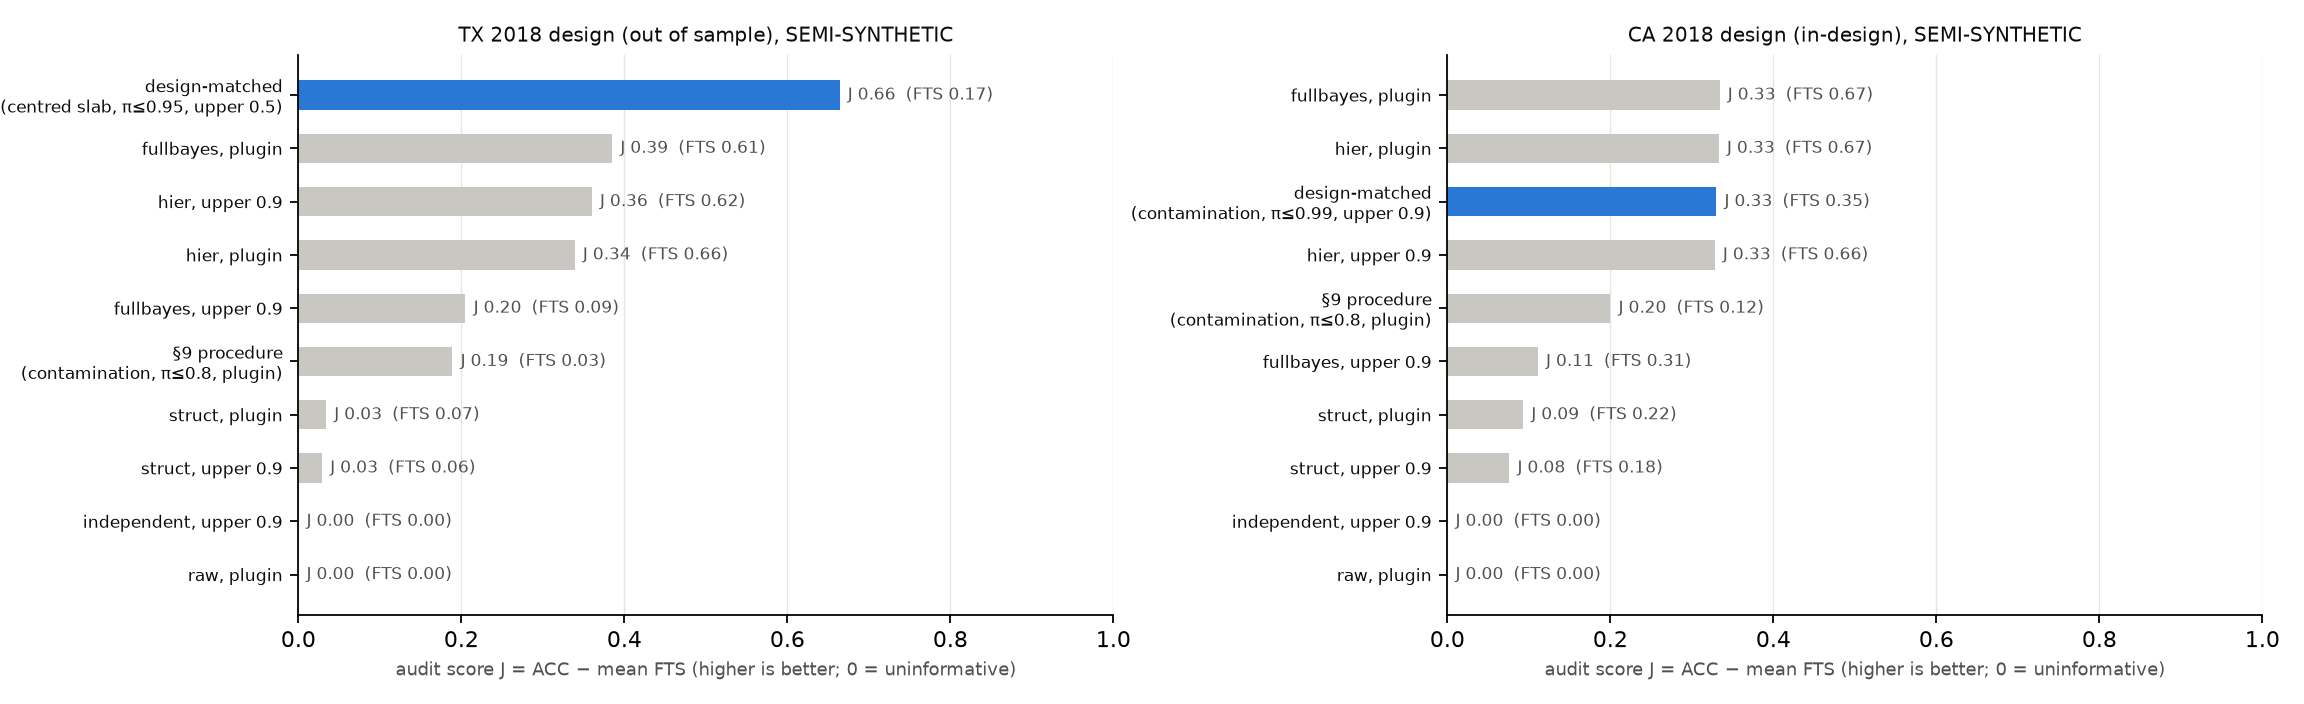
\includegraphics[width=\textwidth]{v2_audit_score.png}
\caption{Audit score $J$ per procedure. Left: Texas design (out of sample). Right: California design (in-design).}\label{fig:v2}
\end{figure}
\begin{table}[t]\centering\small
\caption{Real data: validation-time tolerance claims of the design-matched procedure (5 household splits per state).}\label{tab:v2real}
% generated by make_tables.py from ../results; do not edit by hand
\begin{tabular}{llcccc}
\toprule
State & certification & claims ($\le\epsilon$) & false claims & mean test $\Delta$EOpp & mean test recall \\
\midrule
CA & same-data & 5/5 & 5 & 0.367 & 0.380 \\
CA & held-out & 0/5 & 0 & 0.351 & 0.379 \\
TX & same-data & 5/5 & 5 & 0.238 & 0.350 \\
TX & held-out & 0/5 & 0 & 0.267 & 0.350 \\
\bottomrule
\end{tabular}

\end{table}

\section{Discussion}
\textbf{RQ1.} Pooling masks a disparity when the deficit is confined to a small intersection and is not carried by any
attribute the model pools through. Exchangeable pooling then hides it almost always, and attribute-structured pooling
hides it when it is an interaction. Pooling is harmless when the disparity follows a main effect or involves large groups,
as on real CA data, where the disparity is structural (disability) and huge. The most consequential real-data failure is
selection-time: pooled criteria certified tolerances on validation that did not hold on test.
\textbf{RQ2.} Interval coverage degrades with stronger pooling and smaller groups, and empirical-Bayes plug-in intervals
under-cover even under a correct model. Bayesian credible intervals must not be read as frequentist guarantees.
\textbf{RQ3.} Upper posterior quantiles did not rescue exchangeable pooling, and the invented-design calibration preferred a
posterior-mean rule. Under design-matched calibration, however, upper-quantile rules were chosen in both states, and that
procedure is the best audit out of sample, so posterior uncertainty helps once calibration matches the design. \textbf{RQ4.} No confirmatory difference is robust across bootstrap or refits. The qualitative real-data pattern
replicates in Texas.

\textbf{Limitations.} The struct audit is a restricted version of~\cite{foulds2020bayes}, not an exact reproduction. The
synthetic calibration design is not representative of the real design. Binomial audit likelihoods ignore household
clustering, and the label may contain group-dependent noise~\cite{fogliato2020}. We did not reproduce simultaneous
frequentist bounds~\cite{cherian2024}. Simulated effects are not facts about California.
\textbf{Ethics.} The rule almost never reaches disabled people without public coverage. Pooling can erase a small
group's experience. $\epsilon$ and the capacity were chosen by the analysts, not by the affected communities. No
configuration here is ``fair''; absence of public coverage must not be read as uninsurance or eligibility.

\section{Conclusion}
Bayesian pooling makes intersectional audits more stable, but it can make them falsely reassuring exactly where audits
matter: small intersections whose disadvantage is not explained by any single attribute, and validation-time rule
selection. Auditors should report raw counts, the pooling pull and $P(\Delta>\epsilon)$ together. They should never
certify a tolerance from pooled estimates when intersections have fewer than about 30 positives. Our results support two
concrete practices: calibrate the audit procedure on the design where it will be used (J 0.189 $\to$ 0.664 out of sample),
and certify on data not used to choose the rule (zero false certificates, against 10 of 10 with same-data certification).

\clearpage
% Shared bibliography (\input by literature_review.tex and manuscript.tex). Every entry verified against its
% published abstract or proceedings page.
\begin{thebibliography}{99}\small
\bibitem{foulds2020bayes} J.~R. Foulds, R.~Islam, K.~N. Keya, S.~Pan. Bayesian modeling of intersectional fairness: the variance of bias. \emph{Proc.\ SIAM Int.\ Conf.\ Data Mining (SDM)}, 424--432, 2020. doi:10.1137/1.9781611976236.48. arXiv:1811.07255.
\bibitem{foulds2020icde} J.~R. Foulds, R.~Islam, K.~N. Keya, S.~Pan. An intersectional definition of fairness. \emph{Proc.\ IEEE 36th Int.\ Conf.\ Data Engineering (ICDE)}, 1918--1921, 2020. doi:10.1109/ICDE48307.2020.00203.
\bibitem{kearns2018} M.~Kearns, S.~Neel, A.~Roth, Z.~S. Wu. Preventing fairness gerrymandering: auditing and learning for subgroup fairness. \emph{Proc.\ ICML}, PMLR 80:2564--2572, 2018.
\bibitem{hebert2018} \'U.~H\'ebert-Johnson, M.~P. Kim, O.~Reingold, G.~N. Rothblum. Multicalibration: calibration for the (computationally-identifiable) masses. \emph{Proc.\ ICML}, PMLR 80:1939--1948, 2018.
\bibitem{molina2022} M.~Molina, P.~Loiseau. Bounding and approximating intersectional fairness through marginal fairness. \emph{Advances in NeurIPS 35}, 2022. arXiv:2206.05828.
\bibitem{wang2022} A.~Wang, V.~V. Ramaswamy, O.~Russakovsky. Towards intersectionality in machine learning: including more identities, handling underrepresentation, and performing evaluation. \emph{Proc.\ ACM FAccT}, 336--349, 2022. doi:10.1145/3531146.3533101.
\bibitem{gohar2023} U.~Gohar, L.~Cheng. A survey on intersectional fairness in machine learning: notions, mitigation, and challenges. \emph{Proc.\ IJCAI} (Survey Track), 6619--6627, 2023. doi:10.24963/ijcai.2023/742.
\bibitem{ji2020} D.~Ji, P.~Smyth, M.~Steyvers. Can I trust my fairness metric? Assessing fairness with unlabeled data and Bayesian inference. \emph{Advances in NeurIPS 33}, 18600--18612, 2020. arXiv:2010.09851.
\bibitem{morina2019} G.~Morina, V.~Oliinyk, J.~Waton, I.~Maru\v{s}i\'c, K.~Georgatzis. Auditing and achieving intersectional fairness in classification problems. arXiv:1911.01468, 2019.
\bibitem{lum2022} K.~Lum, Y.~Zhang, A.~Bower. De-biasing ``bias'' measurement. \emph{Proc.\ ACM FAccT}, 379--389, 2022. doi:10.1145/3531146.3533105.
\bibitem{herlihy2024} C.~Herlihy, K.~Truong, A.~Chouldechova, M.~Dud\'ik. A structured regression approach for evaluating model performance across intersectional subgroups. \emph{Proc.\ ACM FAccT}, 2024. arXiv:2401.14893.
\bibitem{himmelreich2025} J.~Himmelreich, A.~Hsu, E.~Veomett, K.~Lum. The intersectionality problem for algorithmic fairness. \emph{Algorithmic Fairness Through the Lens of Metrics and Evaluation}, PMLR 279:68--95, 2025. arXiv:2411.02569.
\bibitem{cherian2024} J.~J. Cherian, E.~J. Cand\`es. Statistical inference for fairness auditing. \emph{Journal of Machine Learning Research} 25(149):1--49, 2024.
\bibitem{hardt2016} M.~Hardt, E.~Price, N.~Srebro. Equality of opportunity in supervised learning. \emph{Advances in NIPS 29}, 3315--3323, 2016.
\bibitem{cotter2019} A.~Cotter, M.~Gupta, H.~Jiang, N.~Srebro, K.~Sridharan, S.~Wang, B.~Woodworth, S.~You. Training well-generalizing classifiers for fairness metrics and other data-dependent constraints. \emph{Proc.\ ICML}, PMLR 97:1397--1405, 2019.
\bibitem{ding2021} F.~Ding, M.~Hardt, J.~Miller, L.~Schmidt. Retiring Adult: new datasets for fair machine learning. \emph{Advances in NeurIPS 34}, 6478--6490, 2021. arXiv:2108.04884.
\bibitem{folktables} Folktables project. Dataset definitions, documentation and data-access tools. \url{https://github.com/socialfoundations/folktables}.
\bibitem{fogliato2020} R.~Fogliato, A.~Chouldechova, M.~G'Sell. Fairness evaluation in presence of biased noisy labels. \emph{Proc.\ AISTATS}, PMLR 108:2325--2336, 2020.
\bibitem{berger1986} J.~O. Berger, L.~M. Berliner. Robust Bayes and empirical Bayes analysis with $\epsilon$-contaminated priors. \emph{Annals of Statistics} 14(2):461--486, 1986. doi:10.1214/aos/1176349933.
\bibitem{datta1995} G.~S. Datta, P.~Lahiri. Robust hierarchical Bayes estimation of small area characteristics in the presence of covariates and outliers. \emph{Journal of Multivariate Analysis} 54(2):310--328, 1995.
\end{thebibliography}


\appendix
\section{Reproducibility}
\textbf{Code and environment.} All analysis is in the executed notebook \nb{}, which runs top to bottom in about
30 minutes on one CPU core. Environment: Python 3.12 with the packages pinned in \texttt{requirements-lock.txt}
(numpy 2.5.4, scipy 1.18.1, pandas 3.1.0, scikit-learn 1.9.1, pgmpy 1.1.2, folktables 0.0.12).
\textbf{Data.} The notebook downloads ACS PUMS 2018 for CA and TX through Folktables. The data are not redistributed.
\textbf{Determinism.} All seeds are fixed (splits 0--4, bootstrap 7, simulations fixed per section); two consecutive
full runs produced identical printed outputs.
\textbf{Commands.}
\begin{verbatim}
uv venv --python 3.12 .venv
uv pip install --python .venv/bin/python -r requirements.txt
.venv/bin/python -m ipykernel install --sys-prefix --name p8
.venv/bin/jupyter nbconvert --to notebook --execute --inplace \
    Problem8_Intersectional_Fairness.ipynb --ExecutePreprocessor.timeout=7200
\end{verbatim}
\textbf{Outputs.} \texttt{results/*.csv} (all tables) and \texttt{figures/*.png}. The tables in this paper are generated
from those CSVs by \texttt{writeup/make\_tables.py}.

\section{Additional tables}
\begin{landscape}
{\footnotesize\setlength{\tabcolsep}{3pt}% generated by make_tables.py from ../results; do not edit by hand
\begin{longtable}{lllcrrrcccccc}
\caption{Intersectional audit table for the BN rule (unconstrained top-30\%, seed-0 test split). $n$ = people, $n^+$ = positives (no public coverage), $k$ = selected positives, TPR = $k/n^+$. Posterior means under each audit model; pull = hier $-$ raw. The contamination column uses $\pi_{\max}=0.95$ because this table is computed (notebook \S7) before the \S9 calibration fixes $\pi_{\max}=0.8$. $\ast$ = exploratory ($<30$ positives or $<30$ negatives).}\label{tab:groups}\\
\toprule
Code & Race (RAC1P) & Sex & Disab. & $n$ & $n^+$ & $k$ & raw TPR & indep. & hier & struct & contam.\,$\pi{\le}0.95$ & pull \\
\midrule
\endfirsthead
\toprule
Code & Race (RAC1P) & Sex & Disab. & $n$ & $n^+$ & $k$ & raw TPR & indep. & hier & struct & contam.\,$\pi{\le}0.95$ & pull \\
\midrule
\endhead
\texttt{7|2|1} & NHPI & F & yes & 4 & 0 & 0 & -- & -- & -- & -- & -- & --\textcolor{red!70!black}{$\ast$} \\
\texttt{4|2|2} & Alaska Native & F & no & 1 & 1 & 0 & 0.000 & 0.324 & 0.129 & 0.000 & 0.137 & 0.129\textcolor{red!70!black}{$\ast$} \\
\texttt{4|2|1} & Alaska Native & F & yes & 2 & 1 & 0 & 0.000 & 0.330 & 0.130 & 0.000 & 0.130 & 0.130\textcolor{red!70!black}{$\ast$} \\
\texttt{4|1|1} & Alaska Native & M & yes & 1 & 1 & 0 & 0.000 & 0.337 & 0.132 & 0.000 & 0.127 & 0.132\textcolor{red!70!black}{$\ast$} \\
\texttt{5|2|1} & AIAN, tribe spec./n.s. & F & yes & 9 & 2 & 0 & 0.000 & 0.248 & 0.105 & 0.006 & 0.104 & 0.105\textcolor{red!70!black}{$\ast$} \\
\texttt{7|1|1} & NHPI & M & yes & 8 & 2 & 0 & 0.000 & 0.252 & 0.103 & 0.033 & 0.105 & 0.103\textcolor{red!70!black}{$\ast$} \\
\texttt{3|2|1} & American Indian & F & yes & 16 & 3 & 0 & 0.000 & 0.197 & 0.085 & 0.005 & 0.080 & 0.085\textcolor{red!70!black}{$\ast$} \\
\texttt{5|1|1} & AIAN, tribe spec./n.s. & M & yes & 14 & 6 & 0 & 0.000 & 0.124 & 0.055 & 0.003 & 0.053 & 0.055\textcolor{red!70!black}{$\ast$} \\
\texttt{3|1|1} & American Indian & M & yes & 20 & 7 & 0 & 0.000 & 0.110 & 0.050 & 0.003 & 0.049 & 0.050\textcolor{red!70!black}{$\ast$} \\
\texttt{5|1|2} & AIAN, tribe spec./n.s. & M & no & 24 & 14 & 1 & 0.071 & 0.127 & 0.088 & 0.100 & 0.088 & 0.017\textcolor{red!70!black}{$\ast$} \\
\texttt{2|2|1} & Black & F & yes & 142 & 21 & 0 & 0.000 & 0.044 & 0.019 & 0.003 & 0.019 & 0.019\textcolor{red!70!black}{$\ast$} \\
\texttt{5|2|2} & AIAN, tribe spec./n.s. & F & no & 37 & 25 & 5 & 0.200 & 0.221 & 0.199 & 0.183 & 0.199 & $-$0.001\textcolor{red!70!black}{$\ast$} \\
\texttt{2|1|1} & Black & M & yes & 187 & 26 & 0 & 0.000 & 0.036 & 0.017 & 0.002 & 0.017 & 0.017\textcolor{red!70!black}{$\ast$} \\
\texttt{9|2|1} & Two or more & F & yes & 77 & 29 & 1 & 0.034 & 0.064 & 0.047 & 0.030 & 0.047 & 0.013\textcolor{red!70!black}{$\ast$} \\
\texttt{9|1|1} & Two or more & M & yes & 97 & 32 & 0 & 0.000 & 0.030 & 0.013 & 0.015 & 0.013 & 0.013 \\
\texttt{7|1|2} & NHPI & M & no & 48 & 32 & 17 & 0.531 & 0.528 & 0.506 & 0.554 & 0.506 & $-$0.025\textcolor{red!70!black}{$\ast$} \\
\texttt{6|1|1} & Asian & M & yes & 125 & 34 & 1 & 0.029 & 0.056 & 0.040 & 0.040 & 0.041 & 0.011 \\
\texttt{7|2|2} & NHPI & F & no & 57 & 38 & 28 & 0.737 & 0.725 & 0.704 & 0.716 & 0.705 & $-$0.032\textcolor{red!70!black}{$\ast$} \\
\texttt{3|1|2} & American Indian & M & no & 84 & 44 & 3 & 0.068 & 0.088 & 0.074 & 0.089 & 0.075 & 0.006 \\
\texttt{8|1|1} & Some other race & M & yes & 209 & 49 & 0 & 0.000 & 0.019 & 0.009 & 0.002 & 0.009 & 0.009 \\
\texttt{3|2|2} & American Indian & F & no & 89 & 55 & 10 & 0.182 & 0.192 & 0.183 & 0.165 & 0.183 & 0.002 \\
\texttt{8|2|1} & Some other race & F & yes & 197 & 56 & 1 & 0.018 & 0.035 & 0.025 & 0.005 & 0.024 & 0.007 \\
\texttt{6|2|1} & Asian & F & yes & 159 & 64 & 5 & 0.078 & 0.091 & 0.083 & 0.077 & 0.082 & 0.005 \\
\texttt{1|1|1} & White & M & yes & 965 & 289 & 3 & 0.010 & 0.014 & 0.012 & 0.012 & 0.012 & 0.002 \\
\texttt{2|2|2} & Black & F & no & 541 & 312 & 31 & 0.099 & 0.102 & 0.100 & 0.114 & 0.100 & 0.001 \\
\texttt{1|2|1} & White & F & yes & 1046 & 365 & 10 & 0.027 & 0.030 & 0.028 & 0.025 & 0.028 & 0.001 \\
\texttt{2|1|2} & Black & M & no & 655 & 377 & 27 & 0.072 & 0.074 & 0.073 & 0.060 & 0.072 & 0.001 \\
\texttt{9|1|2} & Two or more & M & no & 547 & 384 & 149 & 0.388 & 0.389 & 0.387 & 0.362 & 0.386 & $-$0.001 \\
\texttt{9|2|2} & Two or more & F & no & 643 & 450 & 231 & 0.513 & 0.513 & 0.512 & 0.534 & 0.511 & $-$0.001 \\
\texttt{6|1|2} & Asian & M & no & 1488 & 1030 & 634 & 0.616 & 0.615 & 0.615 & 0.602 & 0.614 & 0.000 \\
\texttt{8|1|2} & Some other race & M & no & 1824 & 1139 & 100 & 0.088 & 0.088 & 0.088 & 0.084 & 0.088 & 0.000 \\
\texttt{8|2|2} & Some other race & F & no & 2273 & 1320 & 201 & 0.152 & 0.153 & 0.152 & 0.156 & 0.152 & 0.000 \\
\texttt{6|2|2} & Asian & F & no & 2283 & 1727 & 1288 & 0.746 & 0.745 & 0.745 & 0.753 & 0.745 & $-$0.001 \\
\texttt{1|1|2} & White & M & no & 5805 & 3980 & 1233 & 0.310 & 0.310 & 0.310 & 0.317 & 0.310 & 0.000 \\
\texttt{1|2|2} & White & F & no & 7976 & 5570 & 2734 & 0.491 & 0.491 & 0.491 & 0.486 & 0.491 & 0.000 \\
\bottomrule
\end{longtable}
}
\medskip
\noindent\textbf{Paired bootstrap, seed 0 ($B=1000$).}\par
{\footnotesize% generated by make_tables.py from ../results; do not edit by hand
\begin{tabular}{llcrccc}
\toprule
Comparison & family & metric & estimate & 95\% CI & $p_{\text{boot}}$ & $p_{\text{Holm}}$ \\
\midrule
calibrated $-$ hier plug-in & confirmatory & $\Delta$EOpp & $+0.0000$ & $[+0.0000, +0.0000]$ & 1.000 & 1.000 \\
calibrated $-$ hier plug-in & confirmatory & recall & $+0.0000$ & $[+0.0000, +0.0000]$ & 1.000 & -- \\
calibrated $-$ raw plug-in & confirmatory & $\Delta$EOpp & $-0.0517$ & $[-0.1944, +0.0505]$ & 0.368 & 0.736 \\
calibrated $-$ raw plug-in & confirmatory & recall & $-0.0061$ & $[-0.0089, -0.0035]$ & 0.001 & -- \\
proposed upper $-$ hier plug-in & exploratory & $\Delta$EOpp & $-0.0714$ & $[-0.1755, +0.0000]$ & 0.074 & -- \\
proposed upper $-$ hier plug-in & exploratory & recall & $-0.0026$ & $[-0.0048, -0.0005]$ & 0.014 & -- \\
proposed upper $-$ raw plug-in & exploratory & $\Delta$EOpp & $-0.1231$ & $[-0.3073, +0.0091]$ & 0.076 & -- \\
proposed upper $-$ raw plug-in & exploratory & recall & $-0.0086$ & $[-0.0124, -0.0053]$ & 0.001 & -- \\
struct upper $-$ hier plug-in & exploratory & $\Delta$EOpp & $-0.0714$ & $[-0.1755, +0.0000]$ & 0.074 & -- \\
struct upper $-$ hier plug-in & exploratory & recall & $-0.0026$ & $[-0.0048, -0.0005]$ & 0.014 & -- \\
struct upper $-$ raw plug-in & exploratory & $\Delta$EOpp & $-0.1231$ & $[-0.3073, +0.0091]$ & 0.076 & -- \\
struct upper $-$ raw plug-in & exploratory & recall & $-0.0086$ & $[-0.0124, -0.0053]$ & 0.001 & -- \\
struct plug-in $-$ hier plug-in & exploratory & $\Delta$EOpp & $-0.0714$ & $[-0.1755, +0.0000]$ & 0.074 & -- \\
struct plug-in $-$ hier plug-in & exploratory & recall & $-0.0026$ & $[-0.0048, -0.0005]$ & 0.014 & -- \\
struct plug-in $-$ raw plug-in & exploratory & $\Delta$EOpp & $-0.1231$ & $[-0.3073, +0.0091]$ & 0.076 & -- \\
struct plug-in $-$ raw plug-in & exploratory & recall & $-0.0086$ & $[-0.0124, -0.0053]$ & 0.001 & -- \\
\bottomrule
\end{tabular}
}
\end{landscape}
\end{document}
